\section{Power}
\label{sec:Power}
Fluidic power sources present many challenges for soft robots.
There are three major ways to characterize these power sources: by transmission fluid, circuit continuity, and portability.

\subsection{Transmission Fluids}
Recently, \citet{wehner2014pneumatic} reviewed existing pneumatic energy sources.
However, in general the actuators detailed in Section~\ref{subsec:Actuators, Actuator Morphologies} can be powered using either pneumatic or hydraulic systems where gases or liquids, respectively, are the transmission fluid.
Pneumatics are advantageous for powering FEAs because they provide a low viscosity power transmission medium.
High flows can be achieved with relatively low driving pressures.
However, gases also introduce compressibility into the power transmission system and these dynamics can be difficult to model (refer to \citet{marchese2015control}) and can produce undesirable time delays.
Hydraulics are advantageous because liquids are relatively incompressible when compared to gases, meaning power can be transferred almost immediately from the power source to the actuators.
However, to achieve comparable volumetric flow rates liquid drive systems often require high driving pressures and/or low impedance (large diameter) power transmission lines because of the increased viscosity of the transmission medium.

\subsection{Circuit Continuity}
Further, the actuators detailed in Section~\ref{subsec:Actuators, Actuator Morphologies} can be powered using either open-circuit or closed-circuit power systems.
Open-circuit power systems exhaust the transmission fluid to the environment, whereas closed-circuit systems recover fluid delivered to the actuators.
open-circuit systems are advantageous because they do not require mechanisms to re-pressurize and return transmission fluid to the supply.
However, they often rely on passively exhausting transmission fluid to ambient/environmental pressure meaning the actuator depressurization is unactuated and a function of the actuator's compliance and the impedance of the the exhaust pathway.
Please refer to \citet{marchese2011soft} and \citet{marchese2014autonomous} for examples of open-circuit power systems.
Closed-circuit systems (see Fig.~\ref{fig:tail_actuation_principle}) are advantageous because the amount of transmission fluid is constant and moved around within the system; this means the power system's fluid medium is not required to match the operating environment (e.g., a soft robot fish powered by pneumatics swimming underwater).
Furthermore, because the volume of transmission fluid is constant the power system can typically vacuum fluid from the actuator under power; meaning the system has control authority over actuator depressurization.
The disadvantage to closed-circuit systems is that they typically require additional plumbing to complete the fluid circuit and supporting hardware like a revisable pump.
Please refer to \cite{marchese2014design, katzschmann2014hydraulic} and \cite{marchese2015design} for examples of closed-circuit power systems.

\subsection{Portability}
The portability of a power source may be of significant interest to a soft roboticist.
For example, locomotory soft robots are typically designed under the constraint of being self-contained, meaning all supporting hardware is located onboard the robot.
Additionally, if the untethered robot is intended for high speed maneuvers, then compressed gas \citep{marchese2014autonomous} or combustion \citep{tolley2014untethered} are viable power alternatives.
However, if prolonged operations are required, then open-circuit pumps \citep{tolley2014resilient, onal2013autonomous} or closed-circuit pumps \citep{katzschmann2014hydraulic} are suitable options.
\begin{figure}[htb]
        \centering
            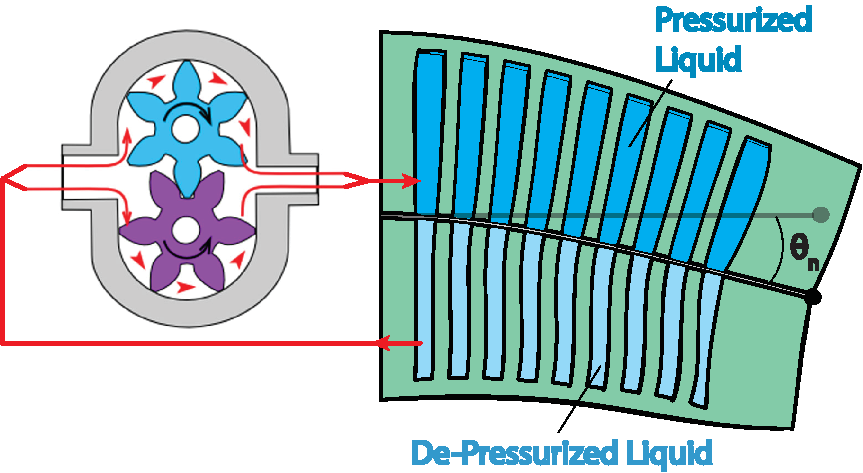
\includegraphics[width=0.85\columnwidth]{figures/power/fish_actuation_principle.pdf}
        \caption[Fish's soft tail actuation principle]{Closed-circuit power system used to drive actuation in the soft hydraulic fish.}
            \label{fig:tail_actuation_principle}
\end{figure}
